\documentclass[11pt]{beamer}
\usepackage[utf8]{inputenc}
\usepackage[T1]{fontenc}
\usetheme{Warsaw}
\begin{document}
	\author{Product owner : Eric Maisel}\label{key}
	\title{PRI - Automne 2018}
	\subtitle{Création de visites  de musée virtuel}
	%\logo{}
	%\institute{}
	\date{}
	%\subject{}
	%\setbeamercovered{transparent}
	%\setbeamertemplate{navigation symbols}{}
	\begin{frame}[plain]
	\maketitle
\end{frame}

\begin{frame}
\frametitle{Objectif}
\begin{block}{}
	\begin{figure}
		\centering
		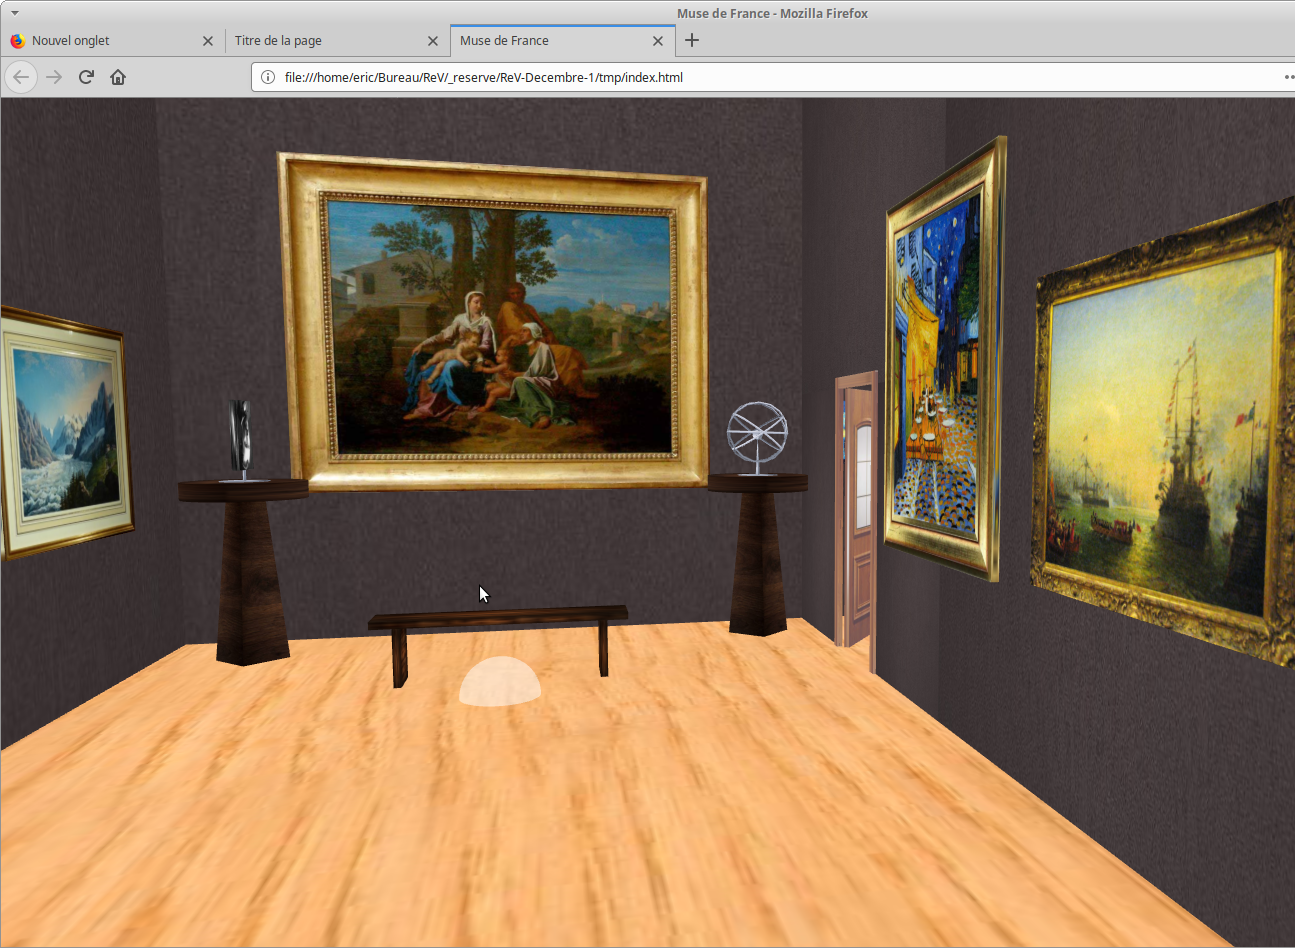
\includegraphics[width=0.9\linewidth]{ima2.jpg}
	\end{figure}
\end{block}
\end{frame}

\begin{frame}
\frametitle{Objectif}
\begin{block}{}
	\begin{figure}
		\centering
		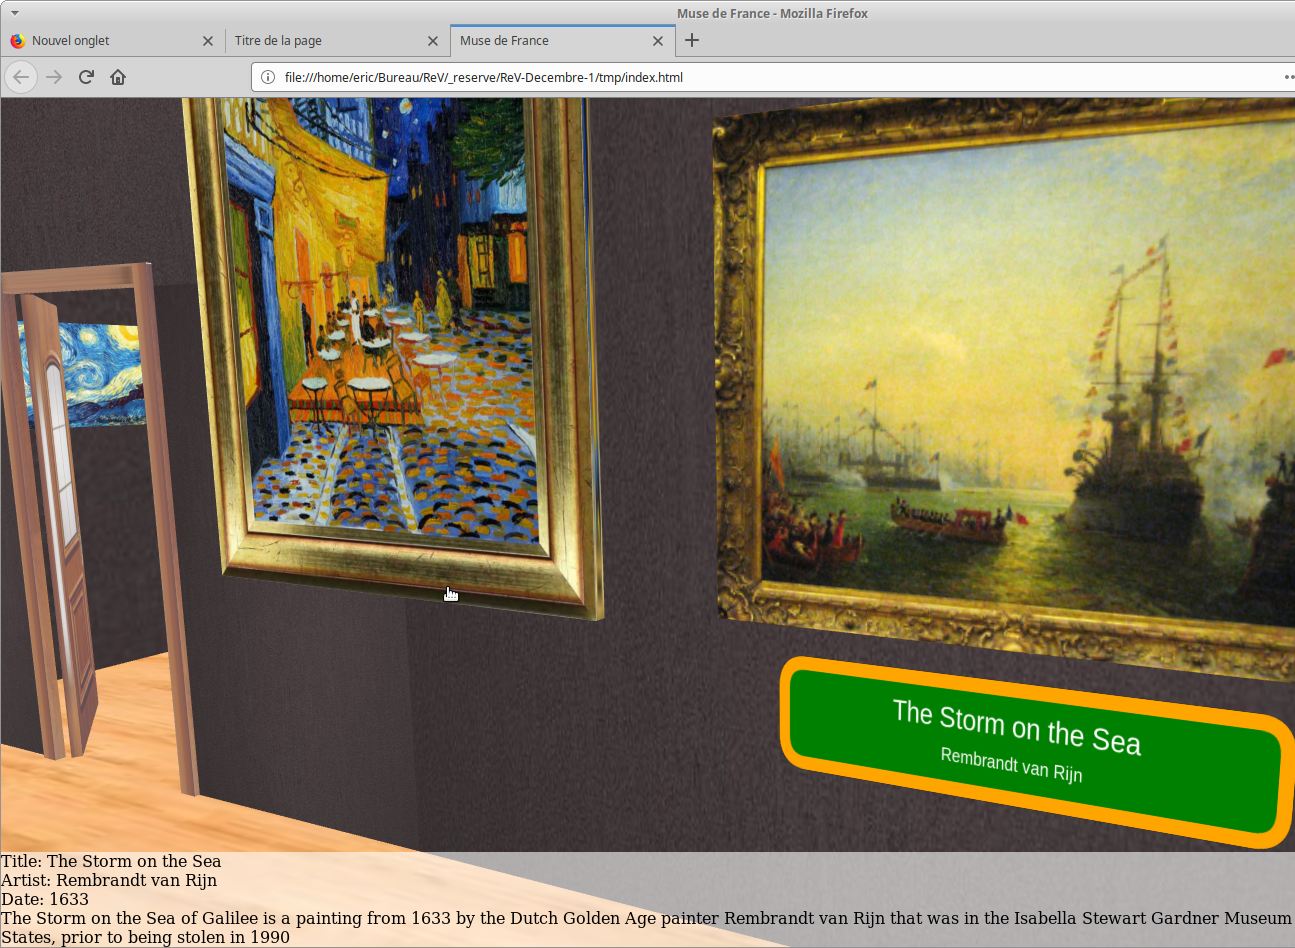
\includegraphics[width=0.9\linewidth]{ima1.jpg}
	\end{figure}
\end{block}
\end{frame}


\begin{frame}
\frametitle{Objectif}
\begin{block}{}
	\begin{figure}
		\centering
		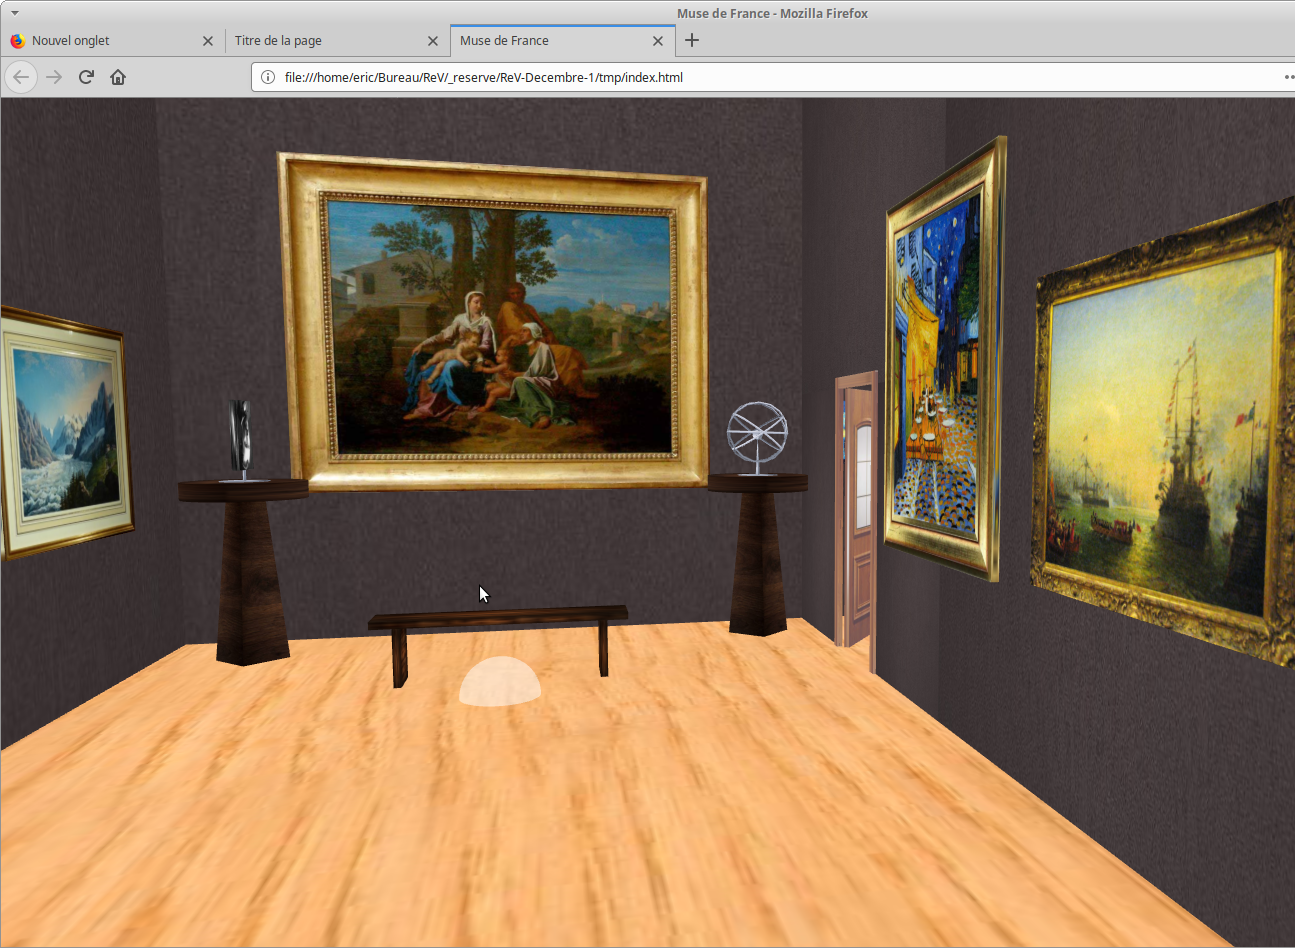
\includegraphics[width=0.45\linewidth]{ima2.jpg}
		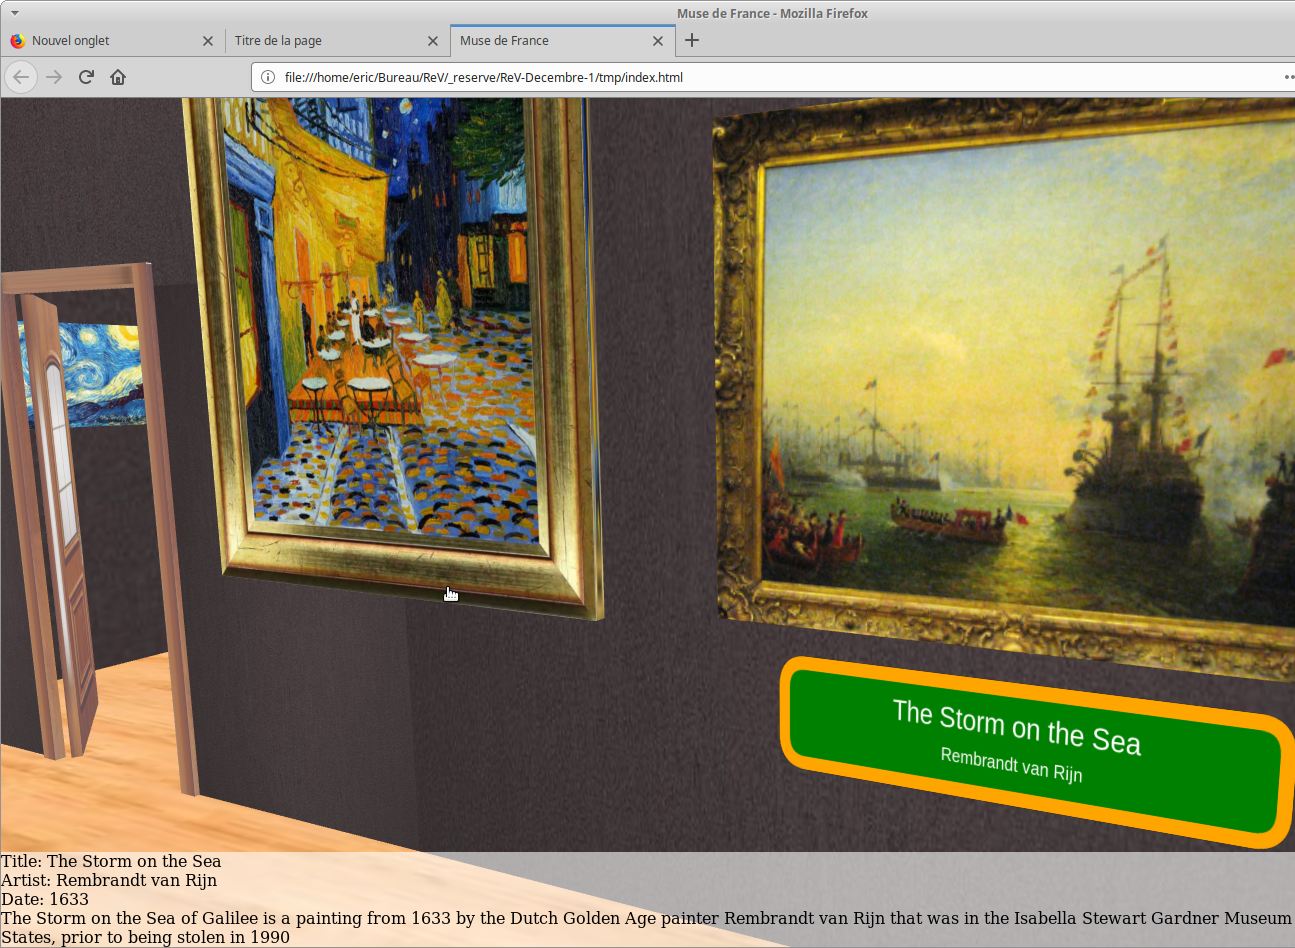
\includegraphics[width=0.45\linewidth]{ima1.jpg}

	\end{figure}
	
\end{block}
\begin{block}{Objectif}
	\begin{itemize}
		\item base de données $\rightarrow$ graphe de scène $\rightarrow$ image interactive
		\item Architecture client / serveur 
		\item Métaphore 3d + Modèle d'attention
		\item Outil auteur 
		\item Programmation modulaire
	\end{itemize}
\end{block}
\end{frame}

\begin{frame}
\frametitle{Structuration}
\begin{block}{Rôle}
	\begin{itemize}
		\item Equipe 
		\item Commissaire d'exposition 
		\item Visiteur 
	\end{itemize}
\end{block}
\begin{block}{Sprints}
	\centering
\begin{tabular}{|c|l|}
	\hline 
	Sprint 0 &  appropriation\\ 
	\hline 
	Sprint 1 &  modèle d'attention\\ 
	\hline 
	Sprint 2 &  génération de scène 3d\\ 
	\hline 
	Sprint 3 &  gestion de grandes quantités de données\\ 
	\hline 
\end{tabular} 
\end{block}
\end{frame}

\begin{frame}
\frametitle{Sprint 0 :appropriation}
\begin{block}{User Stories}
\begin{itemize}
	\item 	US 0.1 : L'{\bf Equipe} sait créer une scène 3d {\bf AFIN} de  comprendre Three.js,
	\item 	US 0.2 : L'{\bf Equipe} sait télécharger depuis un serveur Nodejs des graphes de scène {\bf AFIN} de disposer de plus de flexibilité,
	\item 	US 0.3 : Le {\bf Visiteur } peut se déplacer vers des objets sélectionnés {\bf AFIN} d'explorer le monde 3d.
\end{itemize}
\end{block}

\begin{block}{Livrables}
	\begin{itemize}
		\item Tutoriaux
		\item Logiciel de visualisation 3d
	\end{itemize}
\end{block}
\end{frame}

\begin{frame}
\frametitle{Sprint 1 : modèle d'attention}
\begin{block}{User Stories}
	\begin{itemize}
	\item 	US 1.1 : Le {\bf Visiteur} peut recevoir des informations du tableau qu'il a sélectionné {\bf AFIN}  d'accroître ses connaissances,
\item 	US 1.2 : Le {\bf Visiteur} peut recevoir des informations du tableau auquel il fait attention {\bf AFIN} d'accroître ses connaissances,

\item 	US 1.3 : Le {\bf Visiteur } peut recevoir des informations des tableaux de son voisinage {\bf AFIN} d'accroître ses connaissances,
	\end{itemize}
\end{block}

\begin{block}{Livrables}
	\begin{itemize}
		\item Documentation technique,
		\item Logiciel de visite de musée réactif.
	\end{itemize}
\end{block}
\end{frame}

\begin{frame}
\frametitle{Sprint 2 : génération de scènes 3d}
\begin{block}{User Stories}
	\begin{itemize}
		\item 	US 2.1 : Le {\bf Commissaire d'exposition} peut utiliser  un format de fichier {\bf AFIN} de décrire un musée 3d,
		\item 	US 2.2 : Le {\bf Visiteur} peut charger un fichier décrivant un musée 3d   {\bf AFIN} de pouvoir le visiter.
		\item 	US 3.2 : Le {\bf Commissaire d'exposition} peut appliquer un filtre à une base de données {\bf AFIN} de  décrire un musée 3d.
	\end{itemize}
\end{block}

\begin{block}{Livrables}
	\begin{itemize}
		\item Grammaire du langage de description de scène 3d,
		\item Tutoriels commissaire d'exposition et visiteur,
		\item Documentation technique,
		\item Utilitaires de création de scènes,
		\item Logiciel de visite de musée.
	\end{itemize}
\end{block}
\end{frame}

\begin{frame}
\frametitle{Sprint 3 : gestion de grandes quantités de données}
\begin{block}{User stories}
	\begin{itemize}
		\item U.S 3.1 Le {\bf Commissaire d'exposition} décrit un grand musée .{\bf AFIN} d'avoir une belle démo,
		\item U.S 3.2 Le {\bf Visiteur} peut parcourir un musée qui se télécharge progressivement {\bf AFIN} de réduire la complexité en temps et en espace.
	\end{itemize}
\end{block}
\begin{block}{Livrables}
	\begin{itemize}
		\item Grammaire de l'extension du langage de description,
		\item Documentation technique,
		\item Tutoriel pour le commissaire d'exposition,
		\item Logiciel de visite progressive,
		\item Scène complète.
	\end{itemize}
\end{block}
\end{frame}

\begin{frame}
\frametitle{Ressources}
\begin{block}{Bibliothèques}
	\begin{itemize}
		\item Nodejs
		\item Three.js
		\item Sqlite 
		\item Format JSON
	\end{itemize}
\end{block}

\begin{block}{Langages}
	\begin{itemize}
		\item Javascript
		\item Python
	\end{itemize}
\end{block}
\end{frame}


\end{document}